\documentclass[a4paper,12pt]{article}
\usepackage{amsmath}
\usepackage{graphicx}
\usepackage{bm}

\graphicspath{ {.} }
\begin{document}

\title{%
  The process of minimizing the error function within Machine Learning \\
  \small Mathematics HL Internal Assessment}
\author{Andrew Roberts}
\date{December 2004}
\maketitle
\pagebreak

\section{Neural Networks}
The creation of neural networks comes from the attempts of mimicking the human brain through computation. The process is that given some input x the machine learning algorithm can give an output \(y\), which is the most probable. The neural network setup has three layers. The first layer is the input layer, a matrix \textbf{\emph{X}} of \(i\) inputs \(x_0,x_1,...x_i\).The second layer is the hidden layer where there is a collection of weights and biases manipulated by the machine learning algorithm to introduce the most accurate prediction. The hidden player is anything that is not a part of the other two layers and can be any layers thick. The last layer is the output layer which gives out the output, \(y\). The weights in the hidden layer take on a certain probability value based on a hypothesis function that gets run through an activation function. The collection of values from the previous layer then gets transitioned to the next layer, into each weight and new values are computed. The weights end up making a decision on a regression or classification problem. A regression problem deals with continuous problems, for example deciding the price of a certain size of a new house given data about housing prices and sizes in the region. A classification problem deals with classifying the data. For example, deciding if an image is an apple or an orange. At the output layer, these decisions would be given.

\section{Notation}
The notation \(m\) means the entirety of the training set. \\
The notation \(n\) means the n-th dimension.  \\
The notation \boldmath{$\Theta$}\unboldmath means the parameters of the model.  

\section{Regression}
To go with the example of housing prices, a simple example of a regression problem would be finding a good hypothesis function \(h_\theta(x)\) so that it predicts the price the house sells at. If we take in a single-variable input on the size of the house, the model is linear on the form  \(h_\theta(x) = \theta_0 + \theta_1x\) where the parameters \(\theta_0\) and \(\theta_1\) are the ideal values to minimize an error function, of the notation \(J(\theta\). The goal is that given our training set, \(m\), to learn the hypothesis function. However, given multiple input variables, the model is \(h_\theta(x) = \theta_0x_0 + \theta_1x_1 + ... + \theta_nx_n\).

\section{The error function}
The key to creating accurate models is the error function from the training data. There are multiple ways to represent the error in prediction, but objectively the most popularly used one is the square-error function. The function takes the predicted value and subtracts the accurate value, squaring both. That is done for all of the data from the training set. In mathematical notation, it is noted as
\[J(\theta_0, \theta_1, ..., \theta_n) = \frac{1}{2m} \sum_{i=1}^m (h_\theta(x^{(i)}) - y^{(i)})^2\]
The square-error function is easy to use given its convexity. The function is convex, which means that there is only a single minimum which makes the minimum easy to find. Through minimizing the error function, the ideal parameters can be found, and the model can be applied to be the best fit.

\section{Gradient Descent}
The goal of the gradient descent algorithm is to minimize the error function by using the tangent line at an initial point, and moving into the direction of the negative gradient, toward a local minimum until the gradient is zero at a local minimum. If the function is convex, that point is going to be the global minimum, but if the function is not convex, the reached minimum will depend on the starting point and not necessarily be a global minimum. The algorithm is defined as \[\theta_j = \theta_j - \alpha \frac{\partial}{\partial\theta_j} J(\theta_0, \theta_1, ..., \theta_n)\] The \(\alpha\) marks the learning rate, which gives the difference between the points. A higher learning rate means a bigger jump, which if high enough can result in overshooting the local minimum and failing to converge. A smaller learning rate means the opposite but will be computationally more difficult. The learning rate gets multiplied by the partial derivative of to error function, with respect to the current parameter. The algorithm gets repeated for every parameter at once and moves accordingly. However, to get a complete algorithm, the error function must be partially derived. 
\[J(\theta_0, \theta_1, ..., \theta_n) = \frac{1}{2m} \sum_{i=1}^m (h_\theta(x^{(i)}) - y^{(i)})^2\]
\[\frac{\partial}{\partial\theta_j} [J(\theta_0, \theta_1, ..., \theta_n)] = \frac{\partial}{\partial\theta_j} [\frac{1}{2m} \sum_{i=1}^m (h_\theta(x^{(i)}) - y^{(i)})^2]\]
\[\frac{\partial}{\partial\theta_j} [J(\theta_0, \theta_1, ..., \theta_n)] = \frac{1}{2m} \sum_{i=1}^m \frac{\partial}{\partial\theta_j} [h_\theta(x^{(i)}) - y^{(i)})^2]\]
\[\frac{\partial}{\partial\theta_j} [J(\theta_0, \theta_1, ..., \theta_n)] = \frac{1}{2m} \sum_{i=1}^m 2(h_\theta(x^{(i)}) - y^{(i)}) \frac{\partial}{\partial\theta_j}[h_\theta(x^{(i)}) - y^{(i)}]\]
\[\frac{\partial}{\partial\theta_j} [J(\theta_0, \theta_1, ..., \theta_n)] = \frac{1}{m} \sum_{i=1}^m (h_\theta(x^{(i)}) - y^{(i)})\frac{\partial}{\partial\theta_j} [\theta_0x_0+\theta_1x_1+...+\theta_nx_n-y^{(i)}]\]
\[\frac{\partial}{\partial\theta_j} [J(\theta_0, \theta_1, ..., \theta_n)] = \frac{1}{m} \sum_{i=1}^m (h_\theta(x^{(i)}) - y^{(i)})x_j^{(i)}\]
The final algorithm is therefore
\[\theta_j = \theta_j - \alpha \frac{1}{m} \sum_{i=1}^m (h_\theta(x^{(i)} - y^{(i)})x_j^{(i)} for j = 0,1,...,n\]
The algorithm can be seen in action on this figure. The plot shows the plot of a two feature squared error, plotted against the cost function. The path of the algorithm toward the global minimum is shown in red and blue, for each iteration. 
\\
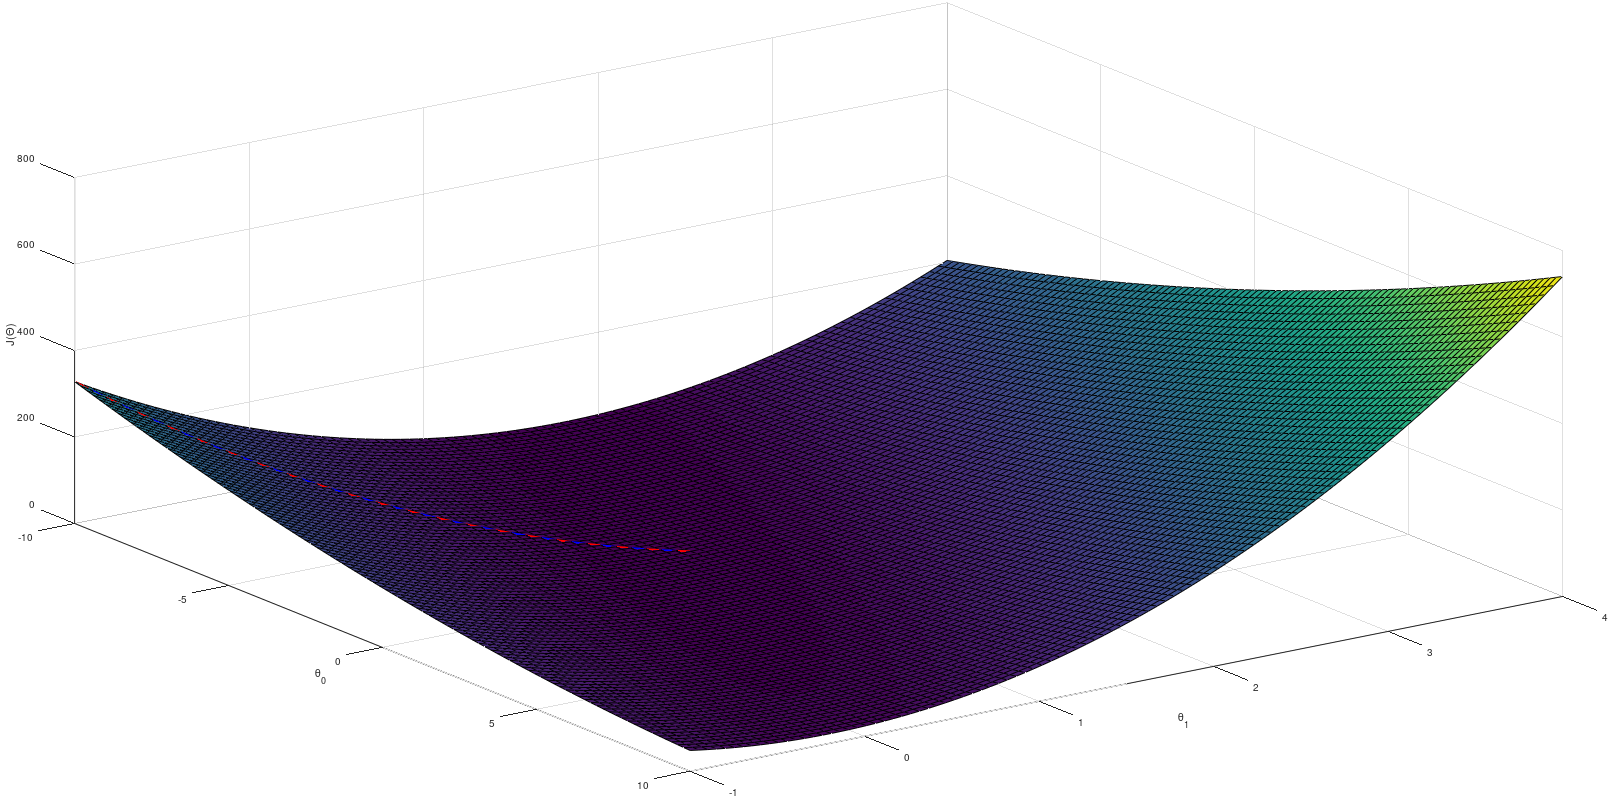
\includegraphics[scale=0.38]{gradientdescent}

\section{Normal equations}
A more analytical way to compute the global minimum of the convex error function is by using normal equations. The normal equation gives the parameters for a minimized error function and is defined as
\begin{center}
\boldmath{$\Theta $}\unboldmath \ $=$ (\boldmath{$X$}\unboldmath$^T$\boldmath{$X$}\unboldmath$)^{-1}$\boldmath{$X$}\unboldmath$^T$\boldmath{$y$}\unboldmath
\end{center}
The theta refers to the matrix containing the minimized \(\theta_j\) values, or weights. The matrix \boldmath{$X$}\unboldmath is the feature dataset, while the matrix \boldmath{$y$}\unboldmath \ is the actual result not predicted by the hypothesis. By taking the squared error function and transform it into a vectorized format:

\[\begin{bmatrix} h_{\boldsymbol{\Theta}} (\boldsymbol{X}^0) - y^0 \\ h_{\boldsymbol{\Theta}} (\boldsymbol{X}^1) - y^1 \\ h_{\boldsymbol{\Theta}} (\boldsymbol{X}^2) - y^2 \\ . \\ . \\ . \\  \\ h_{\boldsymbol{\Theta}} (\boldsymbol{X}^m) - y^m\end{bmatrix}\]

The expression can be split up into two vectors: 
\[\begin{bmatrix} h_{\boldsymbol{\Theta}} (\boldsymbol{X}^0) \\ h_{\boldsymbol{\Theta}} (\boldsymbol{X}^1) \\ h_{\boldsymbol{\Theta}} (\boldsymbol{X}^2) \\ . \\ . \\ . \\ h_{\boldsymbol{\Theta}} (\boldsymbol{X}^m) \end{bmatrix} - \begin{bmatrix} y^0 \\ y^1 \\ y^2 \\ . \\ . \\ . \\ y^m \end{bmatrix}\]
The two vectors can then be simplified, the left one through the identity of the hypothesis function, and the right one given our definition of \boldmath{$y$}\unboldmath:
\[\begin{bmatrix} \boldsymbol{\Theta}^T * \boldsymbol{X}^0 \\ \boldsymbol{\Theta}^T * \boldsymbol{X}^1 \\ \boldsymbol{\Theta}^T * \boldsymbol{X}^2 \\ . \\ . \\ . \\ \boldsymbol{\Theta}^T * \boldsymbol{X}^m \end{bmatrix} - \boldsymbol{y}\]
As the hypothesis function is defined as \(\sum_{i=0}^m \boldsymbol{\Theta}_i x_i\), the vector can be written as:
\[\begin{bmatrix} \boldsymbol{\Theta}_0 * \boldsymbol{X}_0^0 + \boldsymbol{\Theta}_1 * \boldsymbol{X}_1^0 + \boldsymbol{\Theta}_2 * \boldsymbol{X}_2^0 + ... + \boldsymbol{\Theta}_n * \boldsymbol{X}_n^0 \\ \boldsymbol{\Theta}_0 * \boldsymbol{X}_0^1 + \boldsymbol{\Theta}_1 * \boldsymbol{X}_1^1 + \boldsymbol{\Theta}_2 * \boldsymbol{X}_2^1 + ... + \boldsymbol{\Theta}_n * \boldsymbol{X}_n^1 \\ . \\ . \\ . \\ \boldsymbol{\Theta}_0 * \boldsymbol{X}_0^m + \boldsymbol{\Theta}_1 * \boldsymbol{X}_1^m + \boldsymbol{\Theta}_2 * \boldsymbol{X}_2^m + ... + \boldsymbol{\Theta}_n * \boldsymbol{X}_n^m \end{bmatrix} - \boldsymbol{y}\]
The error function can therefore be written as \(\boldsymbol{X\Theta} - \boldsymbol{y}\). To find the square error, the error function can have its terms multiplied by themselves, as so:
\[\frac{1}{2m}(\boldsymbol{X\Theta} - \boldsymbol{y})^T(\boldsymbol{X\Theta} - \boldsymbol{y})\]
Now, to find the minimum \(\boldsymbol{\Theta}\) the expression shall be derived with respect to \(\boldsymbol{\Theta}\) and then solved for \(0\):
\[\frac{\partial}{\partial\boldsymbol{\Theta}}[(\boldsymbol{X\Theta} - \boldsymbol{y})^T(\boldsymbol{X\Theta} - \boldsymbol{y})] = 0\]
The transpose then gets distributed, following the distribution identity \((\boldsymbol{A} + \boldsymbol{B})^T = \boldsymbol{A}^T + \boldsymbol{B}^T\)
\[\frac{\partial}{\partial\boldsymbol{\Theta}}[((\boldsymbol{X\Theta})^T - \boldsymbol{y}^T)(\boldsymbol{X\Theta} - \boldsymbol{y})] = 0\]
Then distributing the parenthesis:
\[\frac{\partial}{\partial\boldsymbol{\Theta}}[(\boldsymbol{X\Theta})^T(\boldsymbol{X\Theta}) - \boldsymbol{y}(\boldsymbol{X\Theta})^T - \boldsymbol{y}^T(\boldsymbol{X\Theta}) - \boldsymbol{y}^T\boldsymbol{y}] = 0\]
Then using the distribution identity again, and collecting like terms given the two vectors are of the same dimensionality:
\[\frac{\partial}{\partial\boldsymbol{\Theta}}[\boldsymbol{X}^T\boldsymbol{\Theta}^T\boldsymbol{X\Theta} - 2\boldsymbol{X}^T\boldsymbol{\Theta}^T\boldsymbol{y} - \boldsymbol{y}^T\boldsymbol{y}] = 0\]
Then splitting the terms and removing the scalar term: 
\[\frac{\partial}{\partial\boldsymbol{\Theta}}[\boldsymbol{X}^T\boldsymbol{\Theta}^T\boldsymbol{X\Theta}] - \frac{\partial}{\partial\boldsymbol{\Theta}}[2\boldsymbol{X}^T\boldsymbol{\Theta}^T\boldsymbol{y}] = 0\]
Evaluating the terms and extracting the scalars:
\[\boldsymbol{X}^T\boldsymbol{X}\frac{\partial}{\partial\boldsymbol{\Theta}}[\boldsymbol{\Theta}^T\boldsymbol{\Theta}] - 2\boldsymbol{X}^T\boldsymbol{y}\frac{\partial}{\partial\boldsymbol{\Theta}}[\boldsymbol{\Theta}^T] = 0 \]
\[2\boldsymbol{X}^T\boldsymbol{X\Theta} - 2\boldsymbol{X}^T\boldsymbol{y} = 0\]
Manipulate the expression with some algebra:
\[2\boldsymbol{X}^T\boldsymbol{X\Theta} = 2\boldsymbol{X}^T\boldsymbol{y}\]
\[\boldsymbol{X}^T\boldsymbol{X\Theta} = \boldsymbol{X}^T\boldsymbol{y}\]
To isolate $\boldsymbol{\Theta}$ the matrix has to be multiplied by its inverse:
\[(\boldsymbol{X}^T\boldsymbol{X})(\boldsymbol{X}^T\boldsymbol{X})^{-1}\boldsymbol{\Theta} = (\boldsymbol{X}^T\boldsymbol{X})^{-1}\boldsymbol{X}^T\boldsymbol{y}\]
\[\boldsymbol{\Theta} = (\boldsymbol{X}^T\boldsymbol{X})^{-1}\boldsymbol{X}^T\boldsymbol{y}\]



























\end{document}
